% !TEX root = ../zeth-protocol-specification.tex

\section{\zeth~statement after primitive instantiation}\label{instantiation:statement}

After instantiating the various primitives and providing security proofs to justify that they comply with the security requirements listed in previous sections, $\RELCIRC$ now becomes:

\begin{itemize}
    \item For each $i \in [\jsin]$:
    \begin{enumerate}
        \item $ \auxinputs.\jsins{i}.\znote.\apk = \blake{2s}{\taggedaddr \concat \pad{0}{\blakeCompLen}}$ \\ with $\taggedaddr$ defined in~\cref{instantiation:prf-comm-crh:prf}
        \item $\auxinputs.\jsins{i}.\nf{} = \blake{2s}{\taggednf \concat \auxinputs.\jsins{i}.\znote.\rho}$ \\ with $\taggednf$ defined in~\cref{instantiation:prf-comm-crh:prf}
        \item $\auxinputs.\jsins{i}.\cm{} = \blake{2s}{\auxinputs.\jsins{i}.\znote.\noter{} \concat \msg}$ \\ with $\msg = \auxinputs.\jsins{i}.\znote.\apk \concat \auxinputs.\jsins{i}.\znote.\rrho \concat \auxinputs.\jsins{i}.\znote.\notev$
        \item $\auxinputs.\htags{i} = \blake{2s}{ \taggedpk \concat \priminputs.\hsig}$ (malleability fix, see~\cref{appendix:trnm}) with $\taggedpk$ defined in~\cref{instantiation:prf-comm-crh:prf}
        \item $(\auxinputs.\jsins{i}.\znote.\notev) \cdot (1 - e) = 0$ is satisfied for the boolean value $e$ set such that if $\auxinputs.\jsins{i}.\znote.\notev > 0$ then $e = 1$.
        \item The Merkle root $\mkroot'$ obtained after checking the Merkle authentication path $\auxinputs.\jsins{i}.\mkpath$ of commitment $\auxinputs.\jsins{i}.\cm{}$, with $\mimcSevenMPPrime{}$, equals to $\priminputs.\mkroot$ if $e = 1$.
        \item $\priminputs.\nfs{i}$ \\ $= \indexedset{\pack{\slice{\auxinputs.\jsins{i}.\nf{}}{k \cdot \bnFieldBitCap}{(k+1) \cdot \bnFieldBitCap}}{\FFx{\rBN}}}{k \in [\floor{\prfNfOutLen/\bnFieldBitCap}]}$
        \item $\priminputs.\htags{i}$ \\ $= \indexedset{\pack{\slice{\auxinputs.\htags{i}}{k \cdot \bnFieldBitCap}{(k+1) \cdot \bnFieldBitCap}}{\FFx{\rBN}}}{k \in [\floor{\prfPkOutLen/\bnFieldBitCap}]}$
    \end{enumerate}
    \item For each $j \in [\jsout]$:
    \begin{enumerate}
        \item $\auxinputs.\znotes{j}.\rrho = \blake{2s}{ \taggedrho \concat \priminputs.\hsig}$ (malleability fix, see~\cref{appendix:trnm}) with $\taggedrho$ defined in~\cref{instantiation:prf-comm-crh:prf}
        \item $\priminputs.\cms{j} = \blake{2s}{\auxinputs.\znotes{j}.\noter{} \concat \msg }$ \\ with $\msg = \auxinputs.\znotes{j}.\apk \concat \auxinputs.\znotes{j}.\rrho \concat \auxinputs.\znotes{j}.\notev$
    \end{enumerate}
    \item $\priminputs.\hsig = \indexedset{\pack{\slice{\auxinputs.\hsig}{k \cdot \bnFieldBitCap}{(k+1) \cdot \bnFieldBitCap}}{\FFx{\rBN}}}{k \in [\floor{\crhhsigOutLen/\bnFieldBitCap}]}$
    \item $\priminputs.\resbits = \packResBits{\indexedset{\auxinputs.\jsins{i}.\nf{}}{i \in [\jsin]}, \auxinputs.\vin, \auxinputs.\vout, \auxinputs.\hsig, \indexedset{\auxinputs.\htags{i}}{i \in [\jsin]}}$
    \item Check that the ``\gls{joinsplit} is balanced'', i.e.~check that the \gls{joinsplit-eq} holds:
    \begin{align*}
        &\pack{\auxinputs.\vin}{\FFx{\rBN}} + \sum_{i \in [\jsin]} \pack{\auxinputs.\jsins{i}.\znote.\notev}{\FFx{\rBN}} \\
        & = \sum_{j \in [\jsout]} \pack{\auxinputs.\znotes{j}.\notev}{\FFx{\rBN}} + \pack{\auxinputs.\vout}{\FFx{\rBN}}
    \end{align*}
\end{itemize}

\begin{remark}
    For higher security, we could use \blake{2b}{} with 32-byte output instead of \sha{256}. In fact, since a precompiled contract computing the \blake{2}{}~compression function~\cite{blakecompietf} has been added to the Istanbul release of \ethereum~(EIP 152~\cite{blake-eip}), it could be possible to write a small wrapper on the smart contracts, in order to hash with \blake{2b}{} with any parameter.
\end{remark}

\subsection{Instantiating the packing functions}\label{instantiation:statement:pack}

As we consider SNARKs based on arithmetic circuits defined over a prime field, all variables in the constraint system are interpreted as field elements. Nevertheless, as illustrated in~\cref{zeth-protocol:statement}, part of the statement consists of functions whose co-domains are sets of binary strings (which may be longer than the bit representation of elements of the finite field). While a bit (i.e.~$\{0, 1\}$) is an element of $\FF_p$ ($p$ prime), it is important to minimize the number of gates in the arithmetic circuit (for proof generation efficiency), and to minimize the number of input wires (to improve verification time). This can be done by representing fragments of binary strings as the base 2 decomposition of field elements, thereby ``packing'' binary strings into multiple elements. Converting binary strings into field elements requires the addition of some arithmetic gates (extending the statement to be proven), but reduces the number of primary inputs (reducing the complexity of the SNARK verification carried out on-chain).
The cost of $\groth$ zk-SNARK~\cite{groth2016size} proof verification is linear in the number of primary inputs, since each input acts as a scalar in a costly scalar multiplication of a curve point in $\gset_1$. Hence, while packing slightly increases the prover cost -- by adding constraints to the circuit -- it simplifies the verifier's work.

In this section, we detail the method by which we encode (resp.~decode) a set of binary strings to (resp.~from) sets of field elements. In the rest of this section, the notion of \emph{packing policy} refers to the set of \emph{packing} and \emph{unpacking} functions.

The set of primary inputs is composed of the input nullifiers, the output commitments, the public values (see~\cite[Section 3.4.3]{zethpaper}) along with the signature hash and the authentication tags for security (malleability fix, see~\cref{appendix:trnm}). The complete description of the public inputs is represented in~\cref{instantiation:eq:primary-inputs}.
%
\begin{equation}\label{instantiation:eq:primary-inputs}
    (\indexedset{\priminputs.\nf{i}}{i \in [\jsin]}, \indexedset{\priminputs.\cms{j}}{j \in [\jsout]}, \vin, \vout, \hsig, \indexedset{\priminputs.\htags{i}}{i \in [\jsin]})
\end{equation}

The primary inputs that consist of binary strings are: the nullifiers $\nfs{}$, the public values $\vin$ and $\vout$, the signature hash $\hsig$ and the authentication tags $\htags{}$.

For a binary string $x$, let $\alpha_x = \ceil{\len{x} / \bnFieldBitCap}$ be the number of field elements required to completely encode $x$ and let $\beta_x = \floor{\len{x} / \bnFieldBitCap}$ be the number of field elements whose capacity is fully used. Let $\gamma_x = \len{x} \pmod{\bnFieldBitCap}$ be the number of ``residual'' bits remaining after fully using $\beta_x$ field elements.

\begin{example}\label{instantiation:eg:packing}
    Consider binary strings $A \in \bin^7$ of length 7, to be encoded over the field $\FFx{41}$. This field has a capacity of $5$ bits, and therefore $\alpha_A = 2$, $\beta_A = 1$, and $\gamma_A = 2$. That is, $A$ can be represented as 2 field elements, or as 1 field element with 2 ``residual'' bits.

    Consider $A = (1111011)$. \cref{instantiation:fig:packingA} illustrates how $A$ can be packed as field elements. Note that the 2 residual bits are taken from the ``beginning'' of the bit string, that is, the highest order bits.
\end{example}

\begin{figure}[ht]
    \centering
    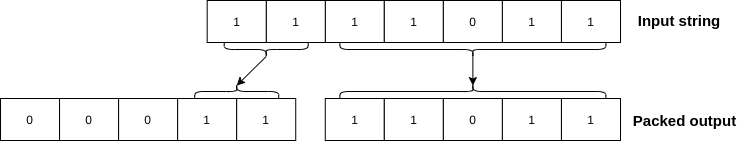
\includegraphics[width=1\textwidth]{images/bit-packing-stringA.png}
    \caption{Packing of string $A$ (see~\cref{instantiation:eg:packing})}\label{instantiation:fig:packingA}
\end{figure}

We now consider strategies to pack all primary inputs that are binary strings. A naive approach is to encode each binary string $x$ as $\alpha_x$ field elements. In general, this results in significant waste (and consequently more field elements than necessary), especially when the number of residual bits is small compared to $\bnFieldBitCap$ (see~\cref{instantiation:fig:packing-multi-strings}). An alternative strategy could be to concatenate all binary strings into a single string $y$ and pack this string into $\alpha_y$ field elements. While this approach minimizes the set of unused bits, each unpack operation would require different shift and mask operations over 2 or 3 field elements. This significantly increases the complexity of the unpacking operation that must be performed on-chain, resulting in a higher gas cost (due to extra logic) or more contract code (if each unpack operation is hard-coded).

The \zeth~protocol requires that each binary string variable $x$ is packed into $\beta_x$ field elements, and the residual bits from all binary strings, along with the public values $\vin$ and $\vout$, are aggregated into a variable $\resbits$. Let $\resBitsBLen$ be the total number of residual bits, and $\resBitsFLen$ be the number of field elements required to represent $\resbits$. We assume that $\zvalueLen < \bnFieldBitCap$, and define the notation $\gamma_\notev = \zvalueLen$ for the bit lengths of public values $\vin$ and $\vout$. Thus $\resBitsBLen$ is given by
\[
    \resBitsBLen = \gamma_\hsig + 2 \cdot \gamma_\notev + \jsin \cdot (\gamma_{\nf{}} + \gamma_{\htag{}} )
\]
and the lengths, in field elements, of each of the correponding public inputs are
\begin{align*}
    \nfFLen &= \beta_{\nf{}} \\
    \hsigFLen &= \beta_{\hsig} \\
    \htagFLen &= \beta_{\htag{}} \\
    \resBitsFLen &= \ceil{\resBitsBLen / \bnFieldBitCap}
\end{align*}

\begin{figure}[ht]
    \centering
    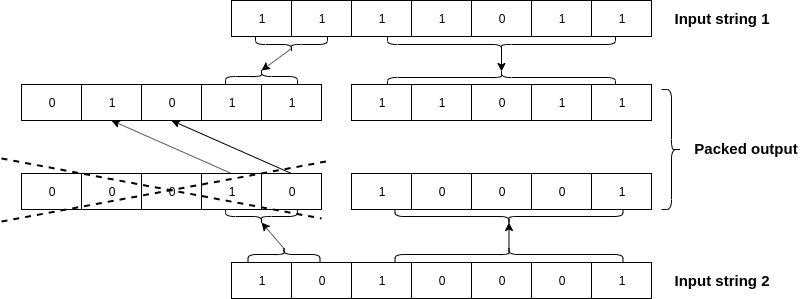
\includegraphics[width=1\textwidth]{images/bit-packing-multi-strings.png}
    \caption{Packing of multiple strings. Observe that, by carefully arranging the bits of the input strings, it is possible to output fewer field elements}\label{instantiation:fig:packing-multi-strings}
\end{figure}

The residual bits $\resbits$ are formatted as follows:
\[
    \widetilde{\hsig} \concat \widetilde{\nfs{}} \concat \widetilde{\htags{}} \concat \vin \concat \vout
\]
where $\widetilde{\hsig}, \widetilde{\nfs{}}, \widetilde{\htags{}}$ are, respectively, the $\gamma_\hsig, \gamma_\nf{}, \gamma_\htag{}$ bits.

Note that the public values are packed into the ``last'', or lowest order, $2 \cdot \gamma_\notev$ bits of the resulting field element(s). In this way, their unpack functions are independent of the values $\jsin$ and $\jsout$ and of the number of residual bits required for each bit string (and consequently, independent of the finite field used).

To format the unpacked primary inputs into field elements, we define the following functions.
Given a bit string of length less than $\bnFieldBitCap$, the algorithm \pack{}{} (see~\cref{zeth-protocol:fig:packing-alg}) returns a field element. Given the nullifiers, public values and authentication tags, the algorithm \packResBits{}{} (see~\cref{zeth-protocol:fig:packing-resbits-alg}) outputs the residual bits. Given a set of packed field elements and the residual bits, the algorithm \unpack{}{} returns the variables reassembled as binary strings. In particular, we have that $\unpack{\priminputs.\nfs{}, \resbits}{\nf{}} = \indexedset{\auxinputs.\jsins{i}.\nf{}}{i \in [\jsin]}$.
\begin{align*}
    &\pack{}{\FFx{\rBN}} : \BB^{\leq \bnFieldBitCap} \to \FFx{\rBN} \\
    &\packResBits{} : {(\BB^\prfNfOutLen)}^{\jsin} \times {(\BB^\zvalueLen)}^2 \times \BB^\crhhsigOutLen \times {(\BB^\prfPkOutLen)}^{\jsin} \to (\FFx{\rBN})^\resBitsFLen \\
    &\unpack{}{} : \FFx{\rBN}^* \times (\FFx{\rBN})^{\resBitsFLen} \to \BB^* \\
\end{align*}

The $\unpack{}{}$ functions for nullifiers, public values and signature hash are represented as follows.
\begin{align*}
    &\unpack{}{}_{\hsig} : (\FFx{\rBN})^\hsigFLen \times (\FFx{\rBN})^{\resBitsFLen} \to \BB^\crhhsigOutLen \\
    &\unpack{}{}_{\nf{}} : (\FFx{\rBN})^\nfFLen \times (\FFx{\rBN})^{\resBitsFLen} \to \BB^\prfNfOutLen \\
    &\unpack{}{}_{\vin} : \FFx{\rBN}^0 \times (\FFx{\rBN})^{\resBitsFLen} \to \BB^\zvalueLen \\
    &\unpack{}{}_{\vout} : \FFx{\rBN}^0 \times (\FFx{\rBN})^{\resBitsFLen} \to \BB^\zvalueLen
\end{align*}

\begin{figure*}
    \begin{minipage}[t]{.4\textwidth}
        \centering
        \procedure{\pack{x}{\FFx{\rBN}}}{%
            out \gets 0_{\FFx{\rBN}}; \\
            \pcfor i \in [\len{x}] \pcdo: \\
            \t \pcif x[i] = 1 \pcdo: \\
            \t \t out \gets out +_{\FFx{\rBN}} 2^{\len{x}-1-i} \\
            \pcreturn out;
        }
        \caption{Algorithm to pack bits into a field element.}\label{zeth-protocol:fig:packing-alg}
    \end{minipage}%
    \begin{minipage}[t]{.6\textwidth}
        \centering
        \procedure{\packResBits{\nfs{}, \vin, \vout, \hsig, \htags{}}}{%
            out \gets []; r \gets \epsilon; \\
            r \gets \vout; \\
            r \gets \vin \concat r; \\
            %
            \pcfor i \in [\jsin] \pcdo:\\
            \t r \gets \slice{\htags{i}}{\beta_{\htags{i}} \cdot \bnFieldBitCap}{} \concat r; \\
            %
            \pcfor i \in [\jsin] \pcdo:\\
            \t r \gets \slice{\nfs{i}}{\beta_{\nfs{i}} \cdot \bnFieldBitCap}{} \concat r; \\
            %
            r \gets \slice{\hsig}{\beta_{\hsig} \cdot \bnFieldBitCap}{} \concat r; \\
            %
            \pcfor i \in [ \ceil{\len{r}/ \bnFieldBitCap} ] \pcdo: \\
            \t out[i] \gets \pack{\slice{r}{i \cdot \bnFieldBitCap}{ (i+1) \cdot \bnFieldBitCap}}{\FFx{\rBN}}; \\
            \pcreturn out;
        }
        \caption{Algorithm to pack residual bits.}\label{zeth-protocol:fig:packing-resbits-alg}
    \end{minipage}
\end{figure*}

\subsubsection{Packing Policy Security}
\begin{proposition}[Packing security]
    For a binary string $x$, it holds that $\unpack{\pack{x}{}}{} = x$ and $\unpack{\packResBits{x}}{} = x$.
\end{proposition}

\subsubsection{Packing Policy Example}

In the case where $\jsin=\jsout=2$, field elements hold $\bnFieldBitCap$ bits and all PRFs and $\crhhsig{}$ output bit-strings of length 256, the unpacked primary inputs are 2167-bit long.
The packing parameters are therefore:
\begin{align*}
    & \resBitsBLen = 143 \\
    & \nfFLen = \hsigFLen = \htagFLen = \resBitsFLen = 1
\end{align*}
The packed primary inputs are 2277 bits long, corresponding to a small space overhead of $\approx 5\%$ unused bits. Moreover, the 143-bit residual bits can be packed into a single field element. As such, the primary inputs are encoded as 9 field elements.
Finally, the residual bits are formatted as follows,
\[
    \underbrace{padding}_{\text{113 bits}}
    \concat \underbrace{\hsig}_{3\ bits}
    \concat \underbrace{\nf{1}}_{3\ bits}
    \concat \underbrace{\nf{0}}_{3\ bits}
    \concat \underbrace{\htag{1}}_{3\ bits}
    \concat \underbrace{\htag{0}}_{3\ bits}
    \concat \underbrace{\vin\vphantom{g}}_{64\ bits}
    \concat \underbrace{\vout\vphantom{g}}_{64\ bits}
\]
